%proof
\section{Proof}\label{sec:proof}

\subsection{Imagen de 3x3}\label{subsec:imagen-de-3x3}

Realizaremos una pequeña prueba con una imagen de 3x3, para ver que el algoritmo funciona correctamente.

La imagen que se va a utilizar para probar el algoritmo es la siguiente:

% centrar la imagen
\includegraphics[width=0.5\textwidth]

Al inicializar la máscara, todos los píxeles pertenecen a la misma clase, por lo que la máscara se inicializa con todos los píxeles con el valor 0.
La máscara es la siguiente matriz:

\begin{equation*}
    \begin{bmatrix}
        0 & 0 & 0 \\
        0 & 0 & 0 \\
        0 & 0 & 0 \\
    \end{bmatrix}
\end{equation*}

Si graficamos la imagen con los valores promedio de todos los píxeles (de esa clase), obtenemos la siguiente imagen:

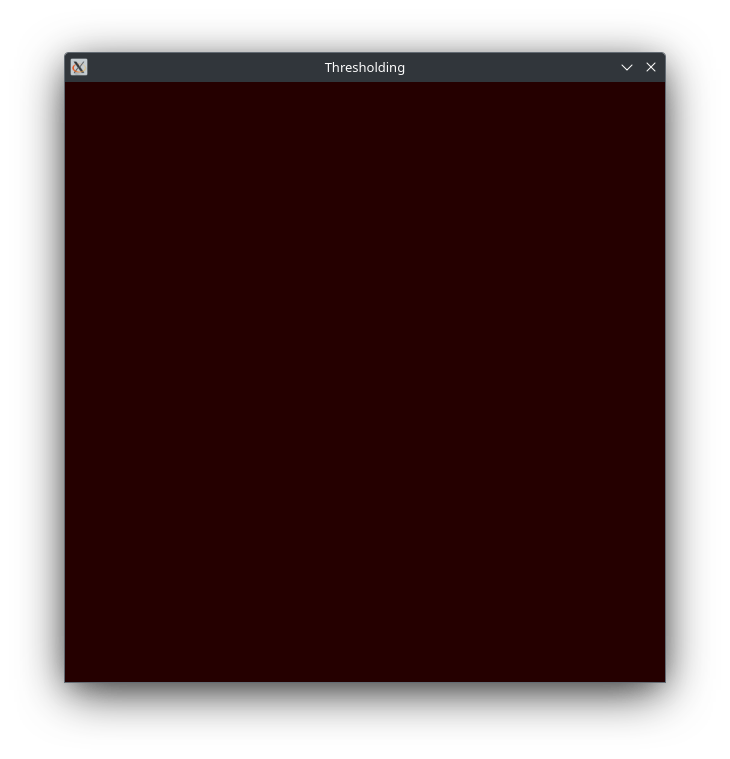
\includegraphics[width=0.5\textwidth]{./latex/img/m0}

Como podemos observar, la imagen tiene todos los píxeles con el mismo valor (promedio de todos los píxeles)

Ahora podemos dividir la clase 0 en 2 clases, luego se realiza la umbralización y se obtiene la siguiente máscara:

\begin{equation*}
    \begin{bmatrix}
        2 & 2 & 1 \\
        2 & 1 & 2 \\
        2 & 2 & 1 \\
    \end{bmatrix}
\end{equation*}

Si graficamos la imagen con los valores promedio de los píxeles de las nuevas clases (1 y 2), obtenemos la siguiente imagen:

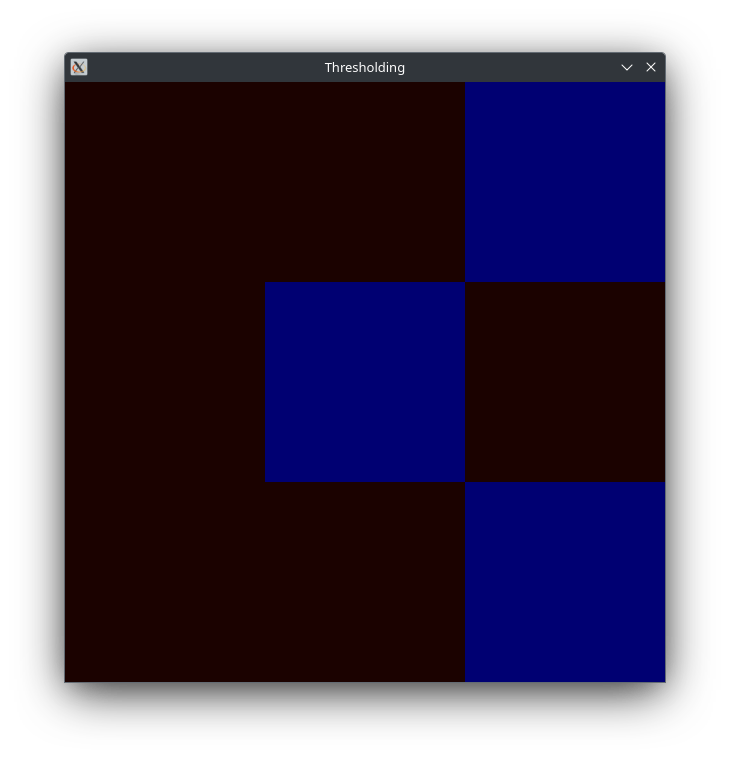
\includegraphics[width=0.5\textwidth]{./latex/img/m1}

Como podemos observar, la imagen se dividió en 2 clases, una con el valor promedio de los píxeles de la clase 1 y otra con el valor promedio de los píxeles de la clase 2.

\begin{equation*}
    \begin{bmatrix}
        5 & 6 & 3 \\
        6 & 4 & 6 \\
        5 & 5 & 3 \\
    \end{bmatrix}
\end{equation*}


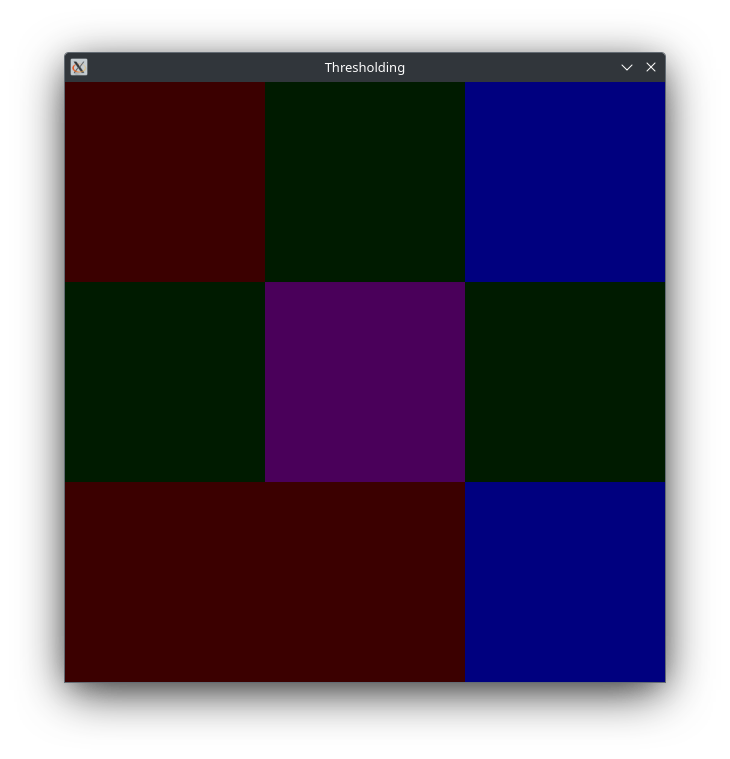
\includegraphics[width=0.5\textwidth]{./latex/img/m2}

\begin{equation*}
    \begin{bmatrix}
        9  & 11 & 7  \\
        12 & 4  & 11 \\
        10 & 9  & 8  \\
    \end{bmatrix}
\end{equation*}

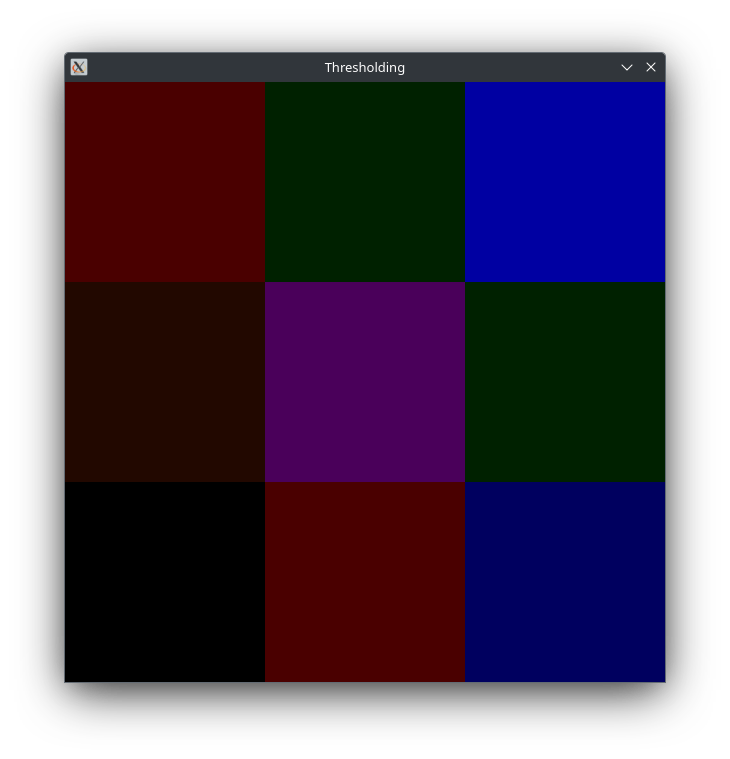
\includegraphics[width=0.5\textwidth]{./latex/img/m3}

\begin{equation*}
    \begin{bmatrix}
        13 & 15 & 7  \\
        12 & 4  & 16 \\
        10 & 14 & 8  \\
    \end{bmatrix}
\end{equation*}

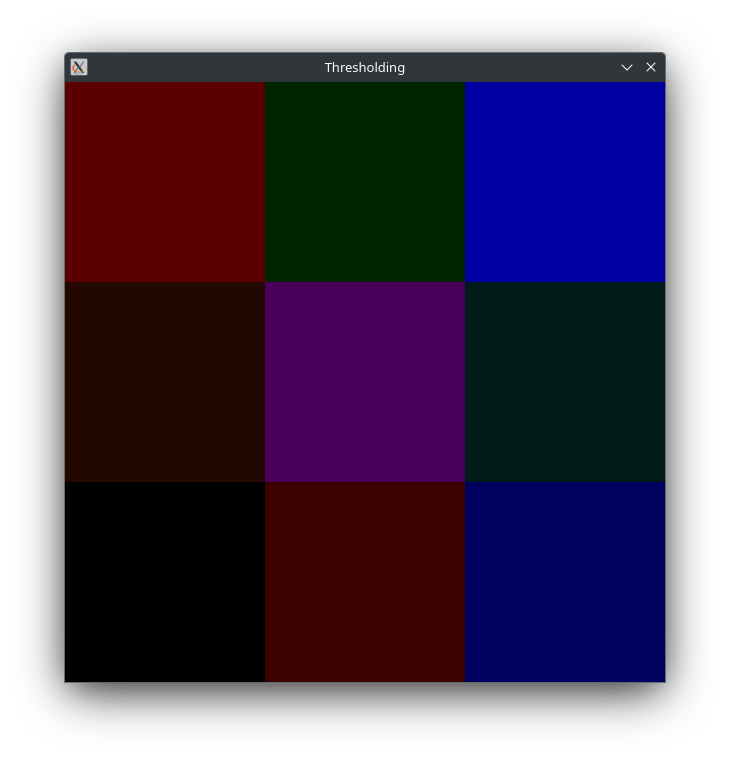
\includegraphics[width=0.5\textwidth]{./latex/img/m4}
